\section{Messwerte und Auswertung}
\label{sec:messwerte}
	
	Für den gesamten Versuch wurden zwei Kristallproben benötigt.
	Abbildung \ref{fig:kristall} zeigt die zweite bereits gespaltete Probe.
	Die erste Probe fiel durch eine zeitweise geringe Haftfähigkeit des Knetwachses von der Halterung im Dunkelraum und war so für immer verloren.

	\begin{figure}[htb]
		\centering
		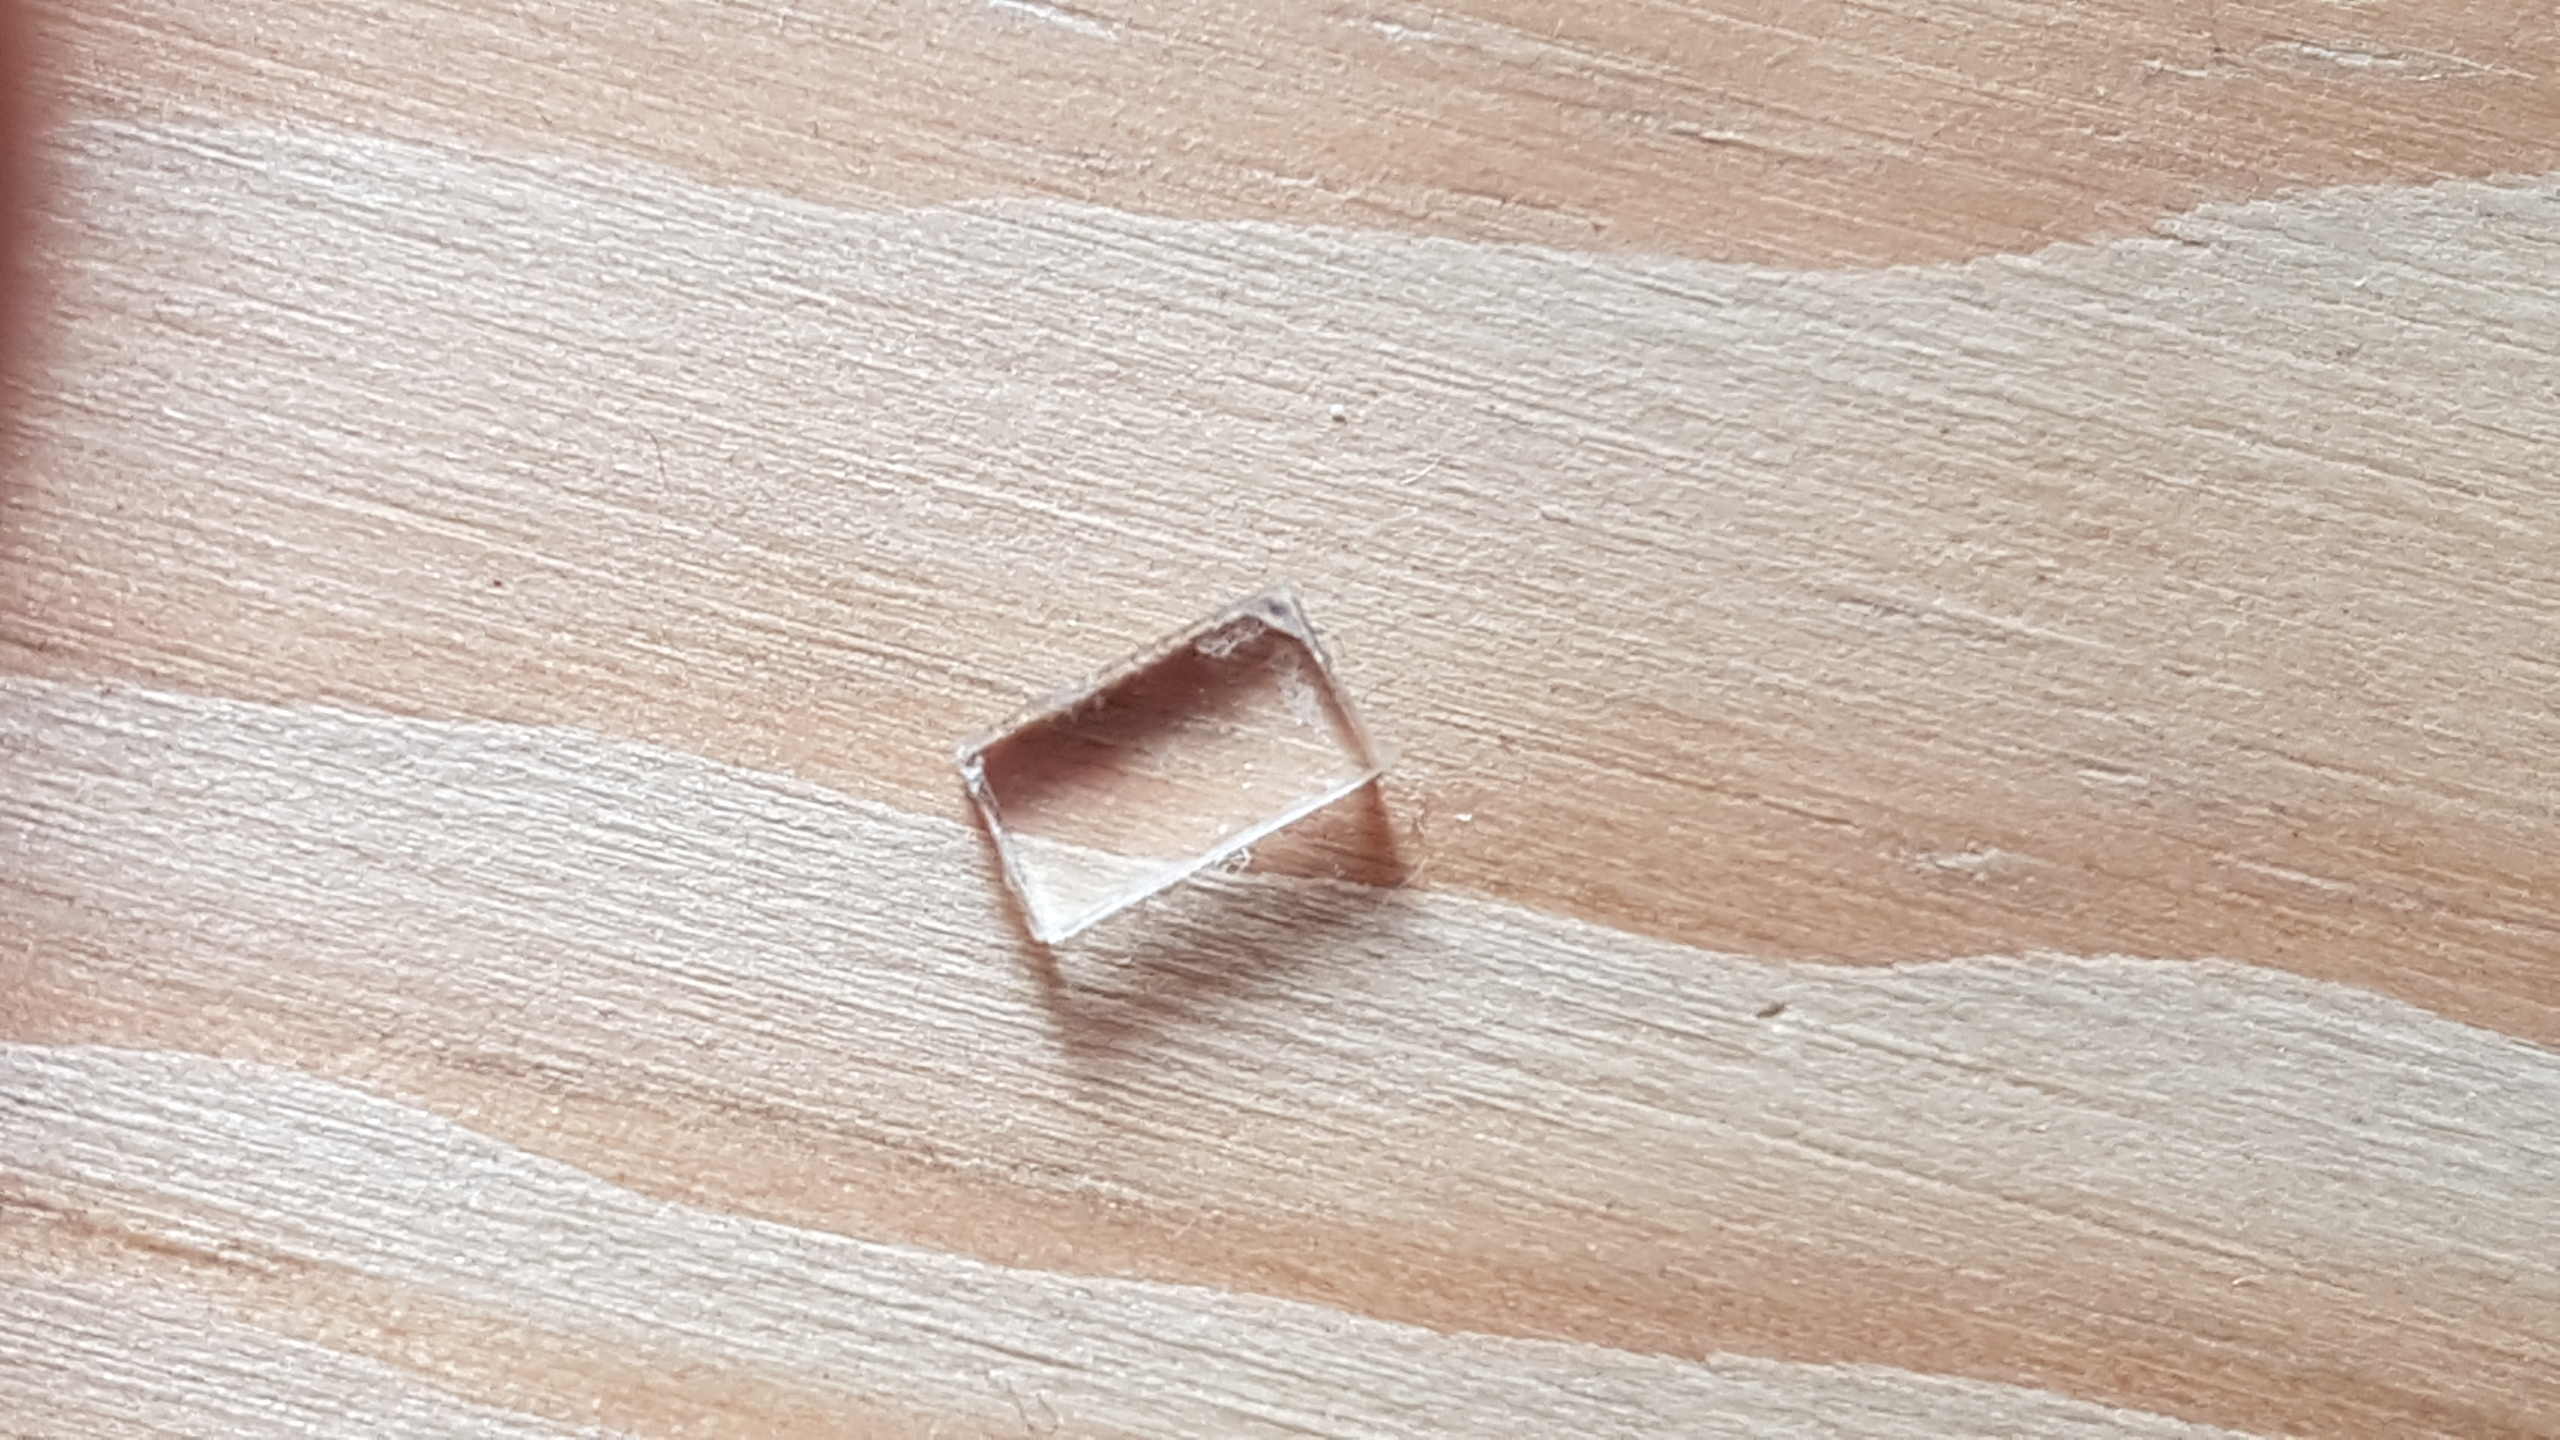
\includegraphics[scale=0.12]{images/20160628_111300.jpg}
		\caption{Aufnahme des verwendeten, bereits gespaltenen Kristalls}
		\label{fig:kristall}
	\end{figure}

	Das gesamte Verfahren zur Belichtung und Auswertung des Röntgenbilds, welches wir in Abschnitt \ref{sec:versuchsaufbau} erläuterten, wurde hier nun vier mal für verschiedene Anoden und Achsen durchgeführt.
	Alle so entstandenen Filme sind in Abbildung \ref{fig:x-ray-film} zu sehen.
	Im Folgenden sei die Auswertung am Beispiel der $(100)$-Achse mit einer Kupfer-Anode als Quelle der Röntgenstrahlung ausführlich erklärt.
	Der Film \ref{fig:cu-100} zeigt diese Aufnahme.

	In allen Aufnahmen stellen die linke Lochblende den Eintritt des Röntgenstrahls in die Kamera und die Rechte dementsprechend den Austritt des Strahls dar.
	Im linken Teilbereich, welcher damit die Reflexion an der Kristalloberfläche darstellt, sind deutliche Streifen zu erkennen.
	Sie lassen sich auf das Vorhandensein von kontinuierlicher Bremsstrahlung zurückführen (siehe Abschnitt \ref{ssub:rntgenbremsstrahlung}).
	Dabei entstehen für jede Wellenlänge verschiedene Reflexe.
	Diese sind alle leicht zueinander versetzt und sehr schwach ausgeprägt im Vergleich zu den Reflexen der $K_\alpha$-Linie des Kupfers.
	Der rechte Teilbereich zeigt keine solche Bremsstrahlungsstreifen.
	Um in diesen Bereich zu gelangen, muss der Röntgenstrahl den Kristall vollständig durchdringen.
	Dies ist aufgrund der eher geringen Intensität der Bremsstrahlung aber nicht möglich, da der Kristall einen großen Anteil der Strahlung absorbiert.

	\begin{figure}[H]
		\begin{subfigure}[b]{\textwidth}
			\centering
			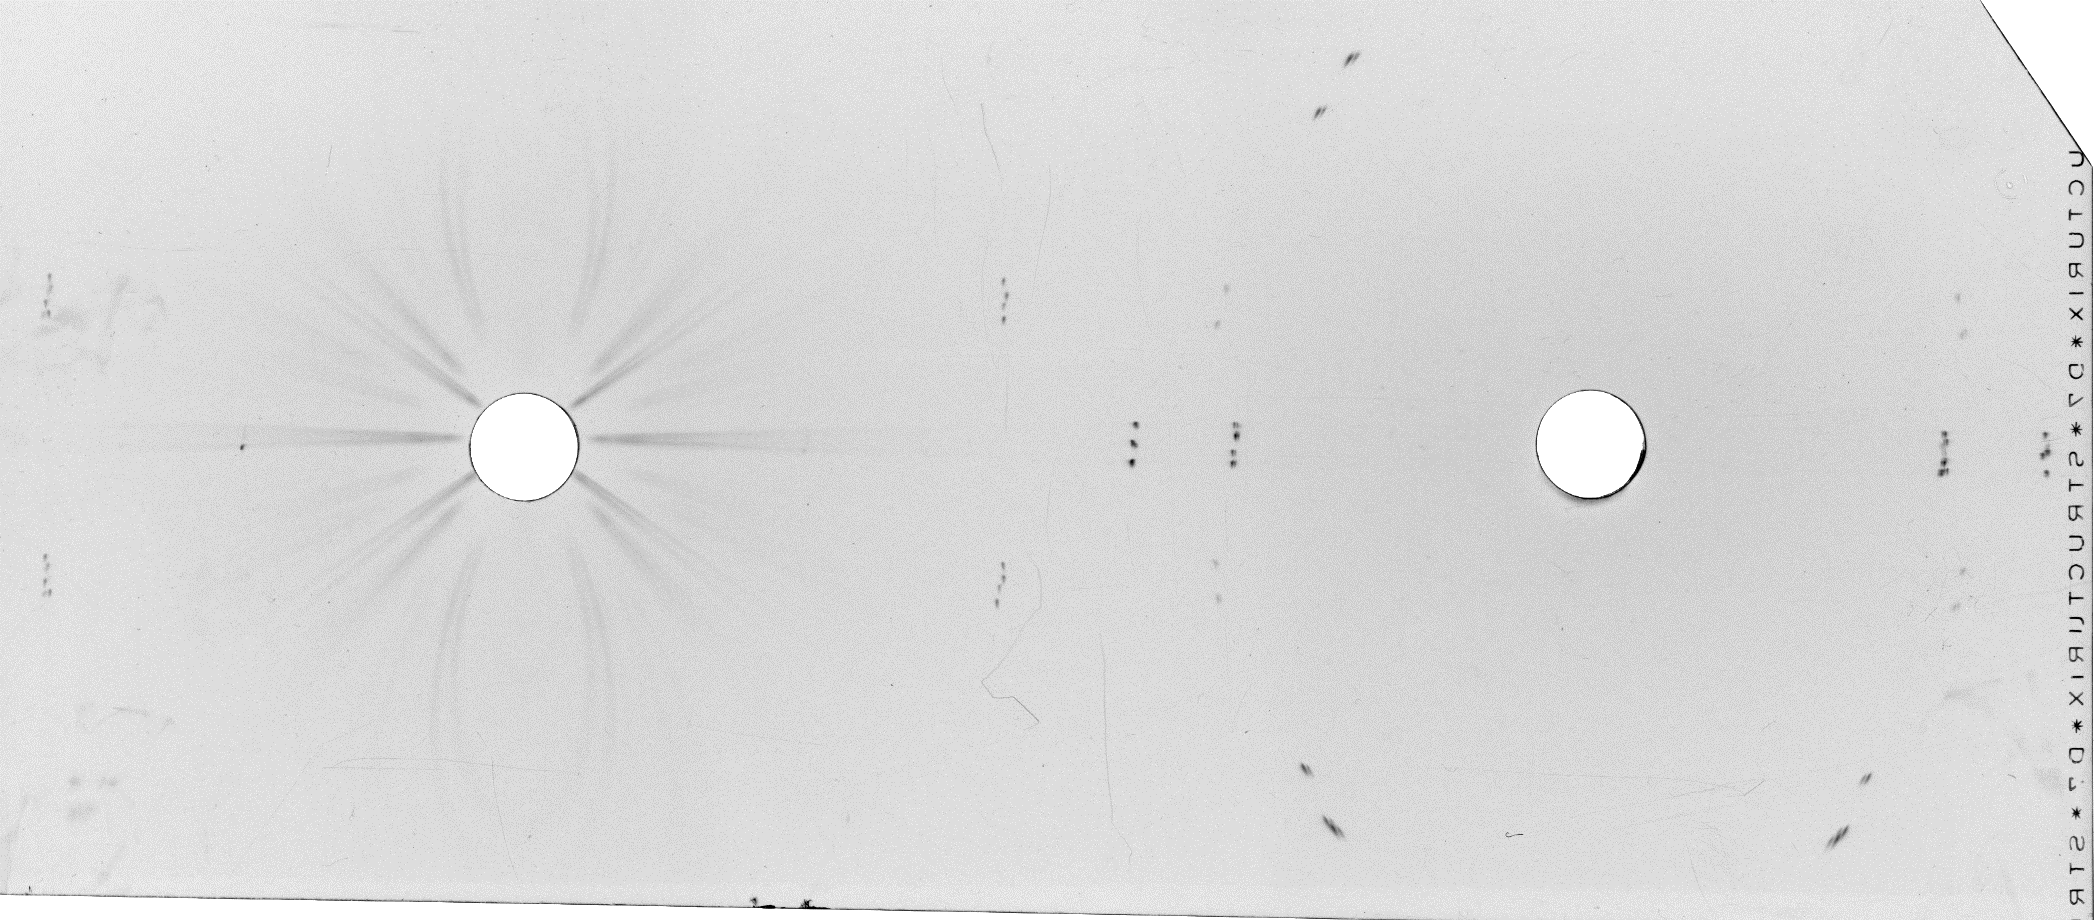
\includegraphics[scale=0.53]{images/cu-100.png}
			\caption{Kupfer-Anode mit Nickel-Filter, $(100)$-Achse}
			\label{fig:cu-100}
		\end{subfigure}

		\begin{subfigure}[b]{\textwidth}
			\centering
			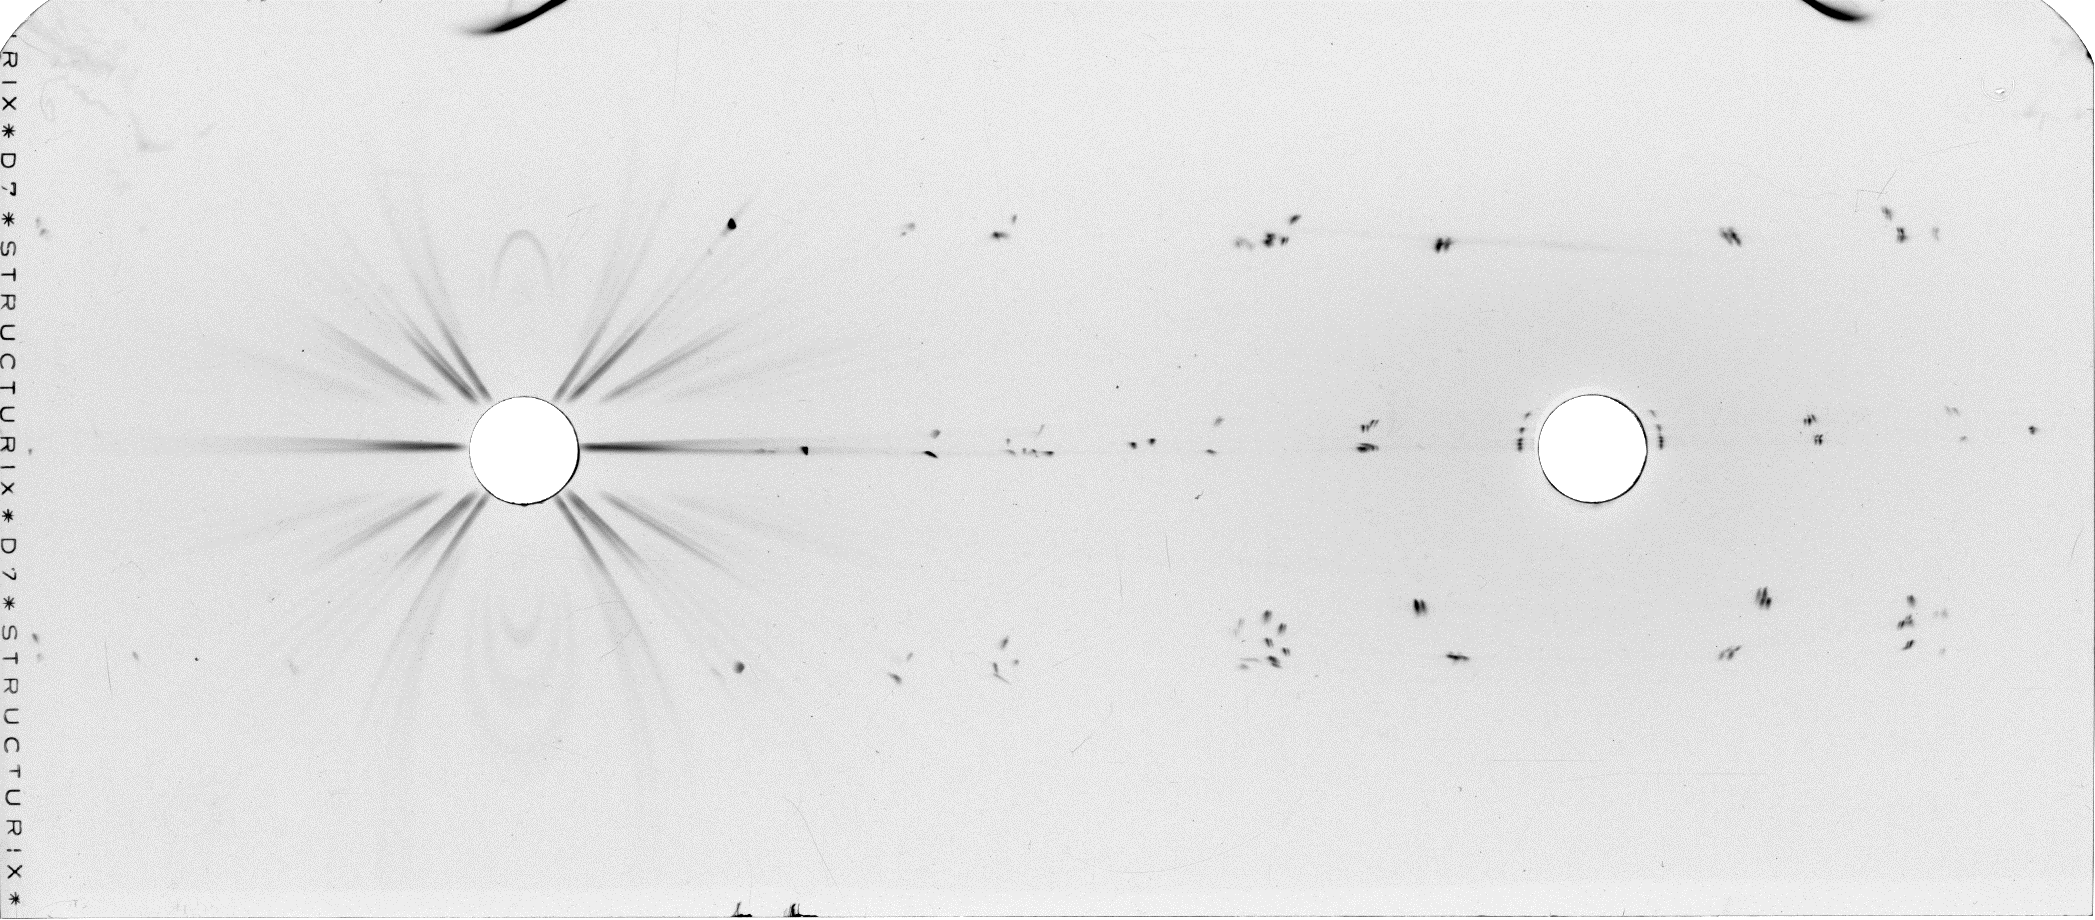
\includegraphics[scale=0.53]{images/cu-110.png}
			\caption{Kupfer-Anode mit Nickel-Filter, $(110)$-Achse}
			\label{fig:cu-110}
		\end{subfigure}

		\begin{subfigure}[b]{\textwidth}
			\centering
			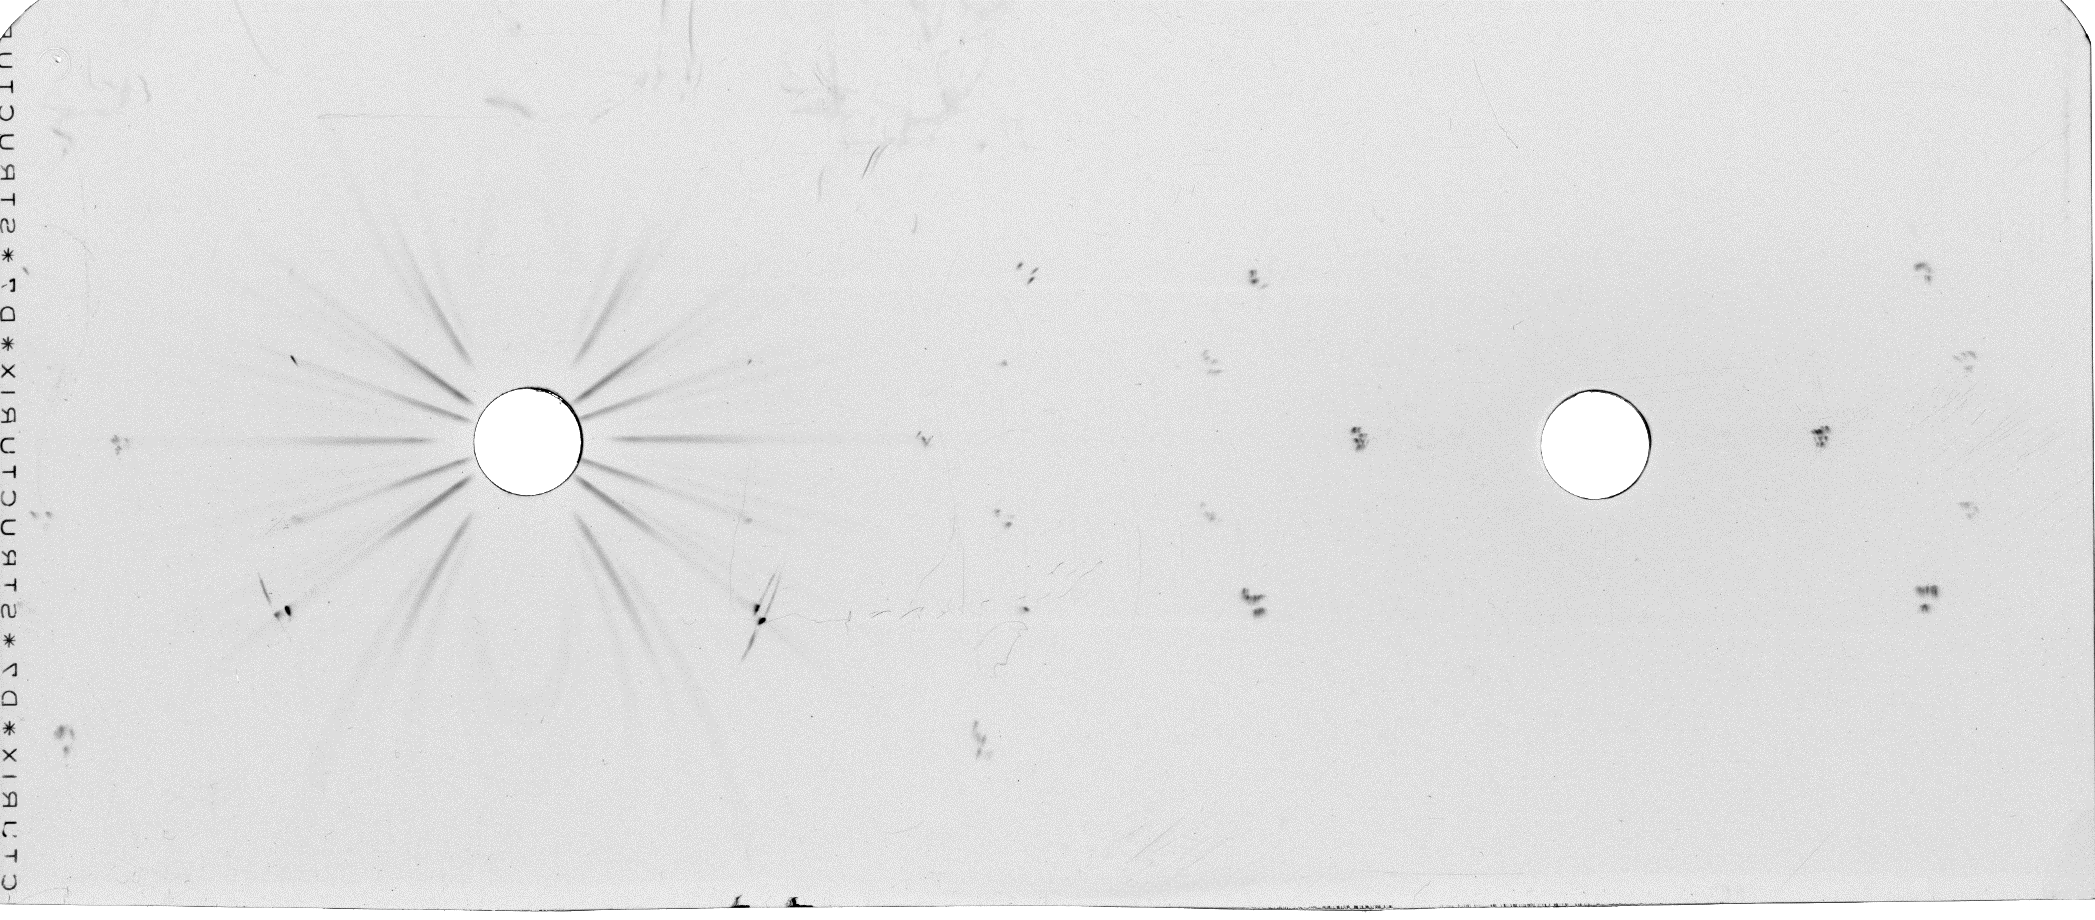
\includegraphics[scale=0.53]{images/cu-111.png}
			\caption{Kupfer-Anode mit Nickel-Filter, $(111)$-Achse}
			\label{fig:cu-111}
		\end{subfigure}

		\begin{subfigure}[b]{\textwidth}
			\centering
			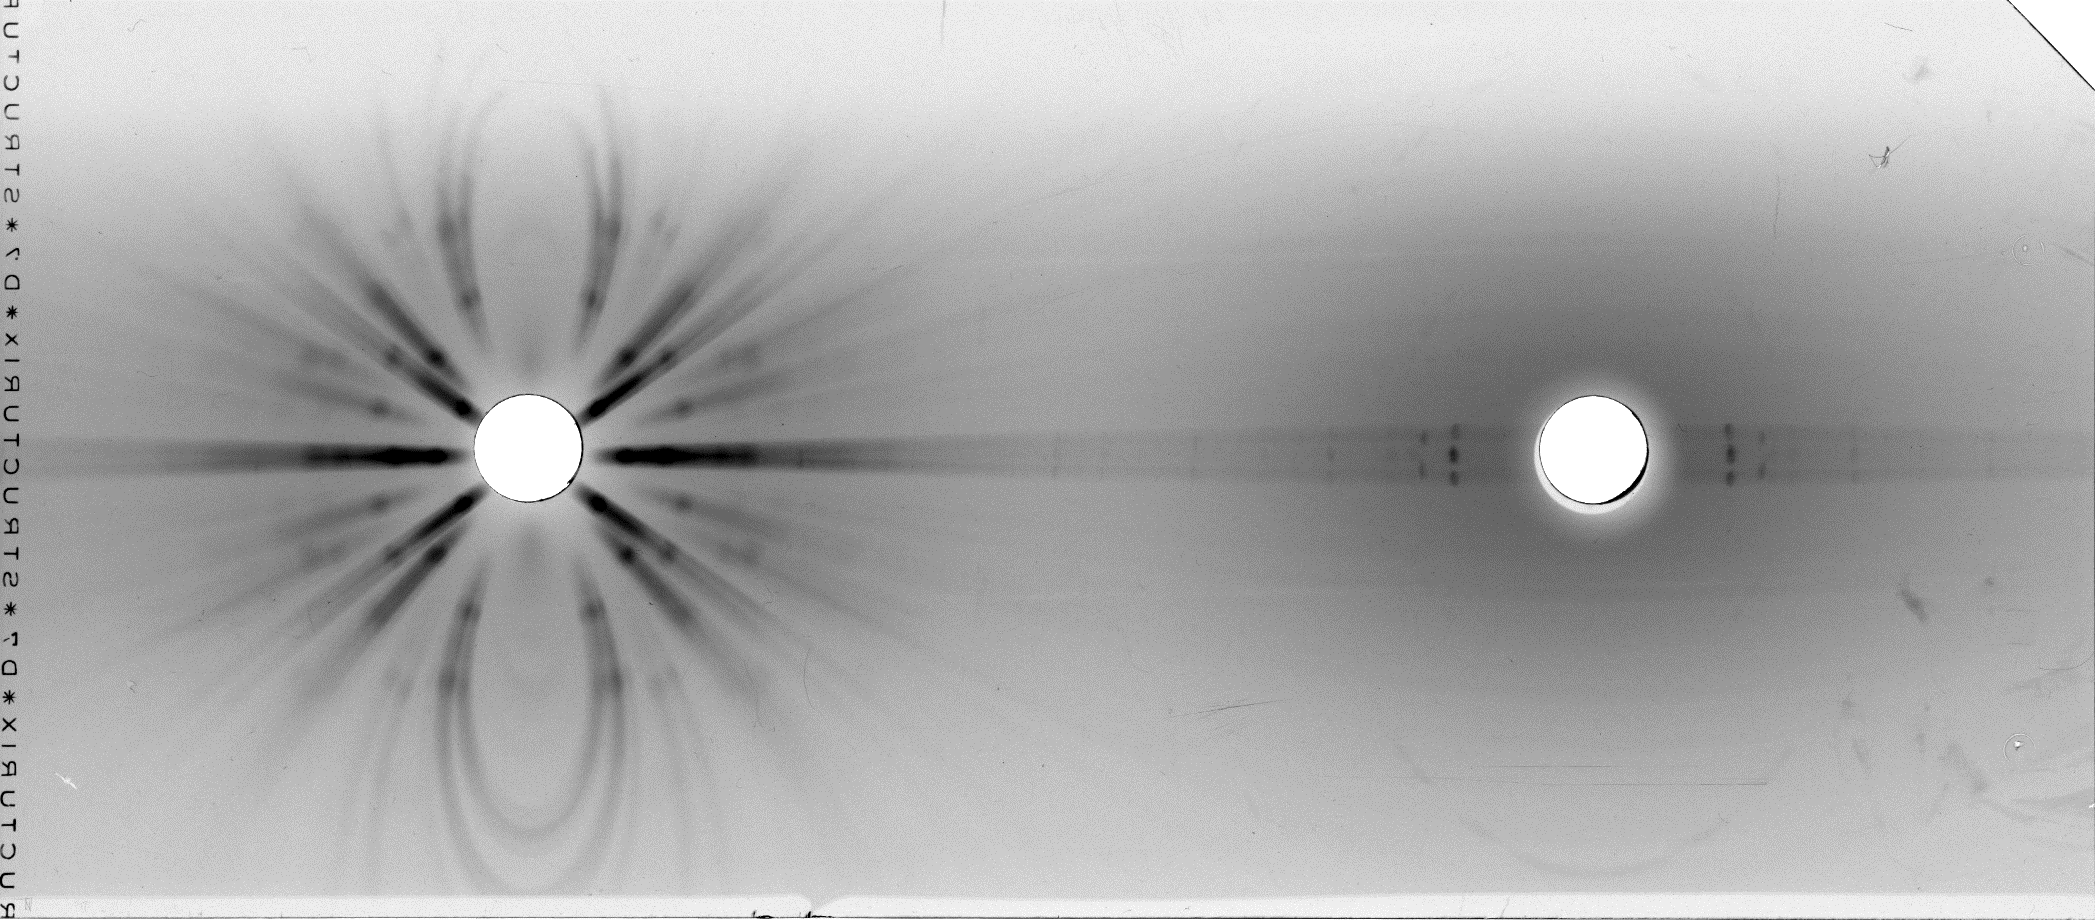
\includegraphics[scale=0.53]{images/ag-100.png}
			\caption{Silber-Anode, $(100)$-Achse}
			\label{fig:ag-100}
		\end{subfigure}
		\caption{aufgenommene Röntgenfilme zu verschiedenen Achsen und Anoden der unbekannten Probe}
		\label{fig:x-ray-film}
	\end{figure}

	Die Bremsstrahlungsstreifen werden durch weitere Reflexe, die ihren Ursprung in der $K_\alpha$-Linie haben, überlagert.
	Diese Reflexe bilden mehrere sogenannte Schichtlinien (siehe Abschnitt \ref{sub:drehkristallverfahren}).
	Als Beispiel sind die Schichtlinien für die $(100)$-Achse mit der Kupfer-Quelle in Abbildung \ref{fig:marker} eingezeichnet.

	\begin{figure}[htb]
		\centering
		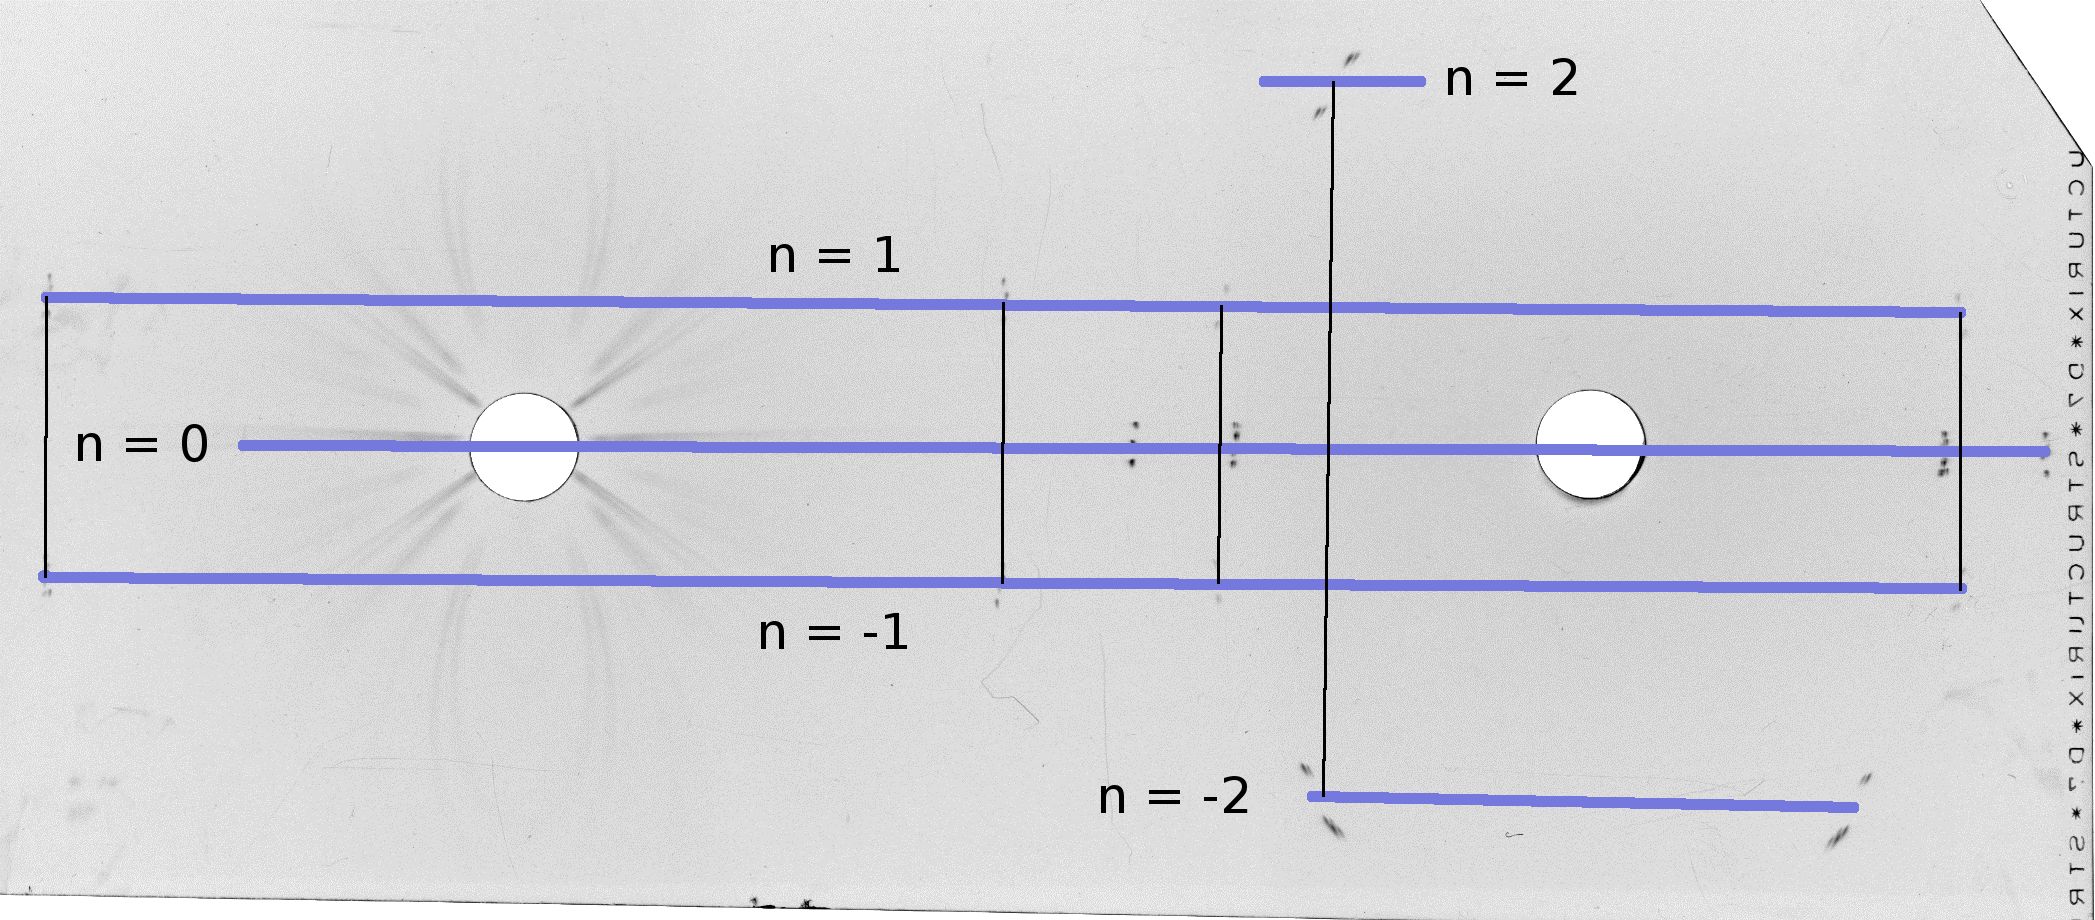
\includegraphics[scale=0.68]{images/cu-100-marker.png}
		\caption{Röntgenfilm mit eingezeichneten Schichtlinien und Abstandsmessungen für die $(110)$-Achse und der Kupfer-Quelle}
		\label{fig:marker}
	\end{figure}

	Für die Bestimmung der Gitterkonstanten und des Kristalltyps ist es nun notwendig die Abstände zwischen diesen Schichtlinien zu bestimmen.
	Aus der Theorie folgt allerdings, dass die Abstände aller zugehöriger Punkte auf den Schichtlinien gleich sein müssen.
	Dies ist für die Reflexe auf dem Röntgenfilm nicht der Fall.
	Aufgrund dieser Tatsache wird im Folgenden immer der Mittelwert aller messbaren Schichtlinienabstände für die Auswertung verwendet.
	Durch Abschätzungen der Minima und Maxima ist damit auch eine Größtfehlerabschätzung möglich.

	In Aufnahme \ref{fig:marker} sind neben der nullten Schichtlinie zwei weitere Schichtlinien zu sehen.
	Diese sind um die Nullte herum symmetrisch verteilt und charakterisieren die Gitterkonstante in Richtung der genannten Drehachse.
	Die Schichtlinien der ersten Ordnung sind im Vergleich zu denen der Zweiten sehr schwach ausgeprägt.
	Dies ist auf den Einfluss des Strukturfaktors zurückzuführen.
	Würde es sich bei dem untersuchten Stoff zum Beispiel um ein flächenzentriertes kubisches Gitter (fcc) bestehend aus einem einzelnem Element handeln, so ist bekannt, dass gewisse ungerade und gerade Reflexe des rein kubischen Gitters sich aufgrund destruktiver Interferenzen aufheben müssen.
	Besteht dieses Gitter aber aus einer Verbindung mehrerer Atome, so ergibt sich, dass eben diese Reflexe nicht voll und ganz verschwinden.

	Bei der Aufnahme \ref{fig:cu-110} der $(110)$-Achse kann damit auch erklärt werden, warum nur die Schichtlinien erster Ordnung zu sehen sind.
	Durch die Drehung der Achse um $45\unit{^\circ}$ werden gerade die flächenzentrierten Gitterpunkte auf die Drehachse projiziert.
	Die Gitterkonstante würde in dieser Richtung also nicht das $\sqrt{2}$-fache der ursprünglichen Gitterkonstante einnehmen, sondern nur das $\sqrt{2}/2$-fache.
	Die Schichtlinien müssen damit weiter auseinander liegen, wodurch die der zweiten Ordnung außerhalb des Films entstehen. 

	Analoge Betrachtungen sind für alle anderen Aufnahmen durchzuführen.
	Es sollen nun die Werte der Gitterkonstanten berechnet werden.

	Es stehe $n$ für die Ordnung einer Schichtlinie und $d_n$ für den jeweiligen Abstand der Schichtlinien dieser Ordnung.
	Für die Messung aller Schichtlinienabstände ergaben sich die in Tabelle \ref{tab:achse-d} gezeigten Werte.
	\begin{table}[H]
		\centering
		\begin{tabular}{r||r|r}
			Achse & $d_1\pm\Delta d_1\ [\unit{cm}]$ & $d_2\pm\Delta d_2\ [\unit{cm}]$ \\
			\hline
			\hline
			$(100)$ & $2.38\pm 0.33$ & $6.05\pm 0.45$ \\
			$(110)$ & $3.50\pm 0.30$ & --- \\
			$(111)$ & $1.25\pm 0.15$ & $2.75\pm 0.15$
		\end{tabular}
		\caption{Schichtlinienabstände der Röntgenfilme aufgenommen durch die Kupfer-Anode}
		\label{tab:achse-d}
	\end{table}

	Aus diesen lassen sich jetzt mit der aus den Grundlagen bekannten Gleichung die Gitterkonstanten der jeweiligen Achsen bestimmen.
	Als Beispiel sei hier die Rechnung für $d_1$ der $(100)$-Achse aufgeführt.
	$a_{(hkl)}$ beschreibe hierbei die Gitterkonstante der $(hkl)$-Achse.
	\[
		a_{(100)} = \frac{n\lambda}{\sin \arctan \frac{d_1}{2r}} = \frac{1.5425 \unit{\AA}}{\sin \arctan \frac{2.38\unit{cm}}{57.5\unit{mm} } } \approx 4.03 \unit{\AA}
	\]
	Wie bereits gesagt, handelt es sich bei den folgenden Fehlertoleranzen um Größtfehlerabschätzungen.
	Sie wurden auf genau dieselbe Art und Weise berechnet, wie $a_{(100)}$.
	Alle berechneten Gitterkonstanten werden in Tabelle \ref{tab:achse-a} aufgeführt.
	\begin{table}[H]
		\centering
		\begin{tabular}{r||r|r|r}
			Achse & $a^{(1)}\pm\Delta a^{(1)}\ [\unit{\AA}]$ & $a^{(2)}\pm\Delta a^{(2)}\ [\unit{\AA}]$ & $\bar{a}\pm\Delta \bar{a}\ [\unit{\AA}]$ \\
			\hline
			\hline
			$(100)$ & $4.03\pm 0.56$ & $4.26\pm 0.17$ & $4.14\pm 0.37$ \\
			$(110)$ & $2.97\pm 0.21$ & --- & $2.97\pm 0.21$ \\
			$(111)$ & $7.26\pm 0.95$ & $7.15\pm 0.34$ & $7.21\pm0.65$
		\end{tabular}
		\caption{berechnete Gitterkonstanten entlang der untersuchten Kristallachsen}
		\label{tab:achse-a}
	\end{table}

	Die somit ermittelten Gitterkonstanten sprechen wieder für eine kubisch flächenzentriertes Kristallgitter (fcc).
	In diesem wäre zu erwarten, dass für die Gitterkonstanten $a_{(hkl)}$ gilt
	\[
		2 \,a_{(110)} = \sqrt{2}\, a_{(100)},\qquad a_{(111)} = \sqrt{3}\, a_{(100)}
	\]
	Demnach sollten die theoretischen Werte $a_{(hkl)}^{\m{th}}$ bei
	\[
		a_{(110)}^{\m{th}} = \curvb{2.93 \pm 0.26}\unit{\AA}, \qquad a_{(111)}^{\m{th}} = \curvb{7.17 \pm 0.64}\unit{\AA}
	\]
	liegen.
	Ein Vergleich mit den Werten aus \ref{tab:achse-d} zeigt eine sehr gute Übereinstimmung im Rahmen des Fehlerintervalls.
	Auch der Fakt, dass die Reflexe mit gemischter Indizierung nur sehr schwach zu sehen sind, spricht stark für eine fcc-Struktur.

	Über die nun ermittelte Gitterkonstante $a_{(100)}$ und die Struktur kann auf die Verbindung geschlossen werden.
	Aus der im Anhang \ref{sec:tabelle} in Abbildung \ref{fig:tab-gitterkonstante} gezeigten Tabelle folgt, dass es sich bei der untersuchten Substanz am wahrscheinlichsten um Lithiumfluorid handelt.
	\[
		a_{(100)}^{\m{m}} = \curvb{4.14 \pm 0.37}\unit{\AA}, \qquad a_{(100)}^{\m{t}} = 4.026 \unit{\AA}
	\]
	Der Stoff war, wie in Abbildung \ref{fig:kristall} zu sehen, durchsichtig und konnte leicht gespalten werden.
	Aus dem bereits Diskutierten kann also geschlossen werden, dass der untersuchte Stoff weder ein Metall noch eine Verbindung aus einem einzigen Elemente sein kann.
	Damit fallen Stoffe wie Platin, Aluminium und Silber, die eine ähnliche Gitterkonstante und den gleichen Bravais-Gittertyp haben, weg.

	Aufnahme \ref{fig:ag-100} zeigt eine weitere Messung, für welche die Silber-Anode ohne einen Filter verwendet wurde.
	Es ist erkennbar, dass mehr Bremsstrahlung sichtbar ist.
	Ohne vorhandenen Filter kann diese natürlich nicht abgeschwächt werden und tritt auf den Aufnahmen verstärkt auf.
	Ebenso sind aber auch doppelt so viele Schichtlinien, wie in den bereits diskutierten vorherigen Fällen zu sehen.
	Dies ist darauf zurückzuführen, dass die effektive Wellenlänge der Röntgenstrahlung bei einer Silber-Anode mit rund $0.5\unit{\AA}$ viel kleiner ist als bei einer Kupfer-Anode mit rund $1.5\unit{\AA}$.
	Fast alle Informationen sind im linken Teilbereich der Aufnahme zu finden.
	Wahrscheinlich absorbiert Lithiumfluorid also die geringere Wellenlänge besser.
	Auch für diese Schichtlinienabstände lässt sich die Gitterkonstante $a_{(100)}$ ermitteln.
	Hierfür soll die Wellenlänge der $K_\alpha$-Linie von Silber mit $\lambda = 0.559\unit{\AA}$ verwendet werden.
	\begin{table}[H]
		\centering
		\begin{tabular}{r||r|r|r|r}
			Ordnung & $1$ & $2$ & $3$ & $4$ \\
			\hline
			% \hline
			Abstände $[\unit{mm}]$ & $8.0$ & $17.0$ & $26.5$ & $38.5$ \\
			\hline
			% \hline
			Gitterkonstante $[\unit{\AA}]$ & $4.06$ & $3.94$ & $4.01$ & $4.02$
		\end{tabular}
		\caption{gemessene und berechnete Werte der $(100)$-Silber-Aufnahme}
		\label{tab:ag-100-val}
	\end{table}
	Die berechneten Gitterkonstanten aus Tabelle \ref{tab:ag-100-val} stimmen mit bereits Berechneten sehr gut überein und lassen ebenfalls auf Lithiumfluorid schließen.
	Der Grund für die gute Übereinstimmung der Werte, obwohl nur die Wellenlänge $K_\alpha$-Linie verwendet wurde, erhält man aus der Tatsache, dass die Intensität der $K_\beta$-Linie von Silber nur rund ein Fünftel der Intensität der $K_\alpha$-Linie beträgt.\footnote{siehe \url{http://xdb.lbl.gov/Section1/Table_1-3.pdf}}
	Ohne den vorhandenen Filter geht die $K_\beta$-Linie im Rauschen der Bremsstrahlung unter.
	Die Röntgenstrahlung kann also immer noch näherungsweise als monochromatisch gesehen werden.

	Auch der Intensitätsverlauf der Bremsstrahlungsstreifen lässt sich auswerten.
	Im Diagramm \ref{fig:spec} ist der bearbeitete Verlauf der Schwärzung entlang der nullten Schichtlinie für einen kleinen Ausschnitt um das Austrittsfenster gezeigt.
	Die genaue Position des untersuchten Gebiets kann man in Abbildung \ref{fig:ausschnitt} sehen.

	\begin{figure}[htb]
		\centering
		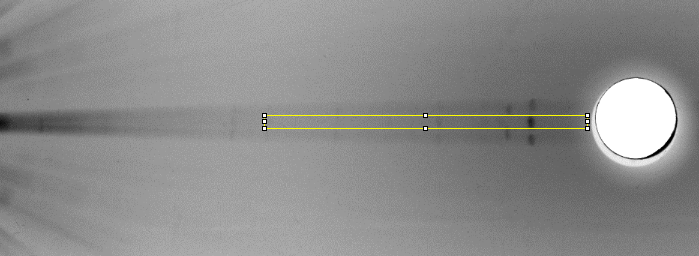
\includegraphics[scale=0.5]{images/ausschnitt.png}
		\caption{Vergrößerter Bereich des Röntgenfilms der $(100)$-Achse und der Silber-Quelle mit markiertem Bereich}
		\label{fig:ausschnitt}
	\end{figure}

	\begin{figure}[htb]
		\centering
		% GNUPLOT: LaTeX picture with Postscript
\begingroup
  \makeatletter
  \providecommand\color[2][]{%
    \GenericError{(gnuplot) \space\space\space\@spaces}{%
      Package color not loaded in conjunction with
      terminal option `colourtext'%
    }{See the gnuplot documentation for explanation.%
    }{Either use 'blacktext' in gnuplot or load the package
      color.sty in LaTeX.}%
    \renewcommand\color[2][]{}%
  }%
  \providecommand\includegraphics[2][]{%
    \GenericError{(gnuplot) \space\space\space\@spaces}{%
      Package graphicx or graphics not loaded%
    }{See the gnuplot documentation for explanation.%
    }{The gnuplot epslatex terminal needs graphicx.sty or graphics.sty.}%
    \renewcommand\includegraphics[2][]{}%
  }%
  \providecommand\rotatebox[2]{#2}%
  \@ifundefined{ifGPcolor}{%
    \newif\ifGPcolor
    \GPcolorfalse
  }{}%
  \@ifundefined{ifGPblacktext}{%
    \newif\ifGPblacktext
    \GPblacktexttrue
  }{}%
  % define a \g@addto@macro without @ in the name:
  \let\gplgaddtomacro\g@addto@macro
  % define empty templates for all commands taking text:
  \gdef\gplbacktext{}%
  \gdef\gplfronttext{}%
  \makeatother
  \ifGPblacktext
    % no textcolor at all
    \def\colorrgb#1{}%
    \def\colorgray#1{}%
  \else
    % gray or color?
    \ifGPcolor
      \def\colorrgb#1{\color[rgb]{#1}}%
      \def\colorgray#1{\color[gray]{#1}}%
      \expandafter\def\csname LTw\endcsname{\color{white}}%
      \expandafter\def\csname LTb\endcsname{\color{black}}%
      \expandafter\def\csname LTa\endcsname{\color{black}}%
      \expandafter\def\csname LT0\endcsname{\color[rgb]{1,0,0}}%
      \expandafter\def\csname LT1\endcsname{\color[rgb]{0,1,0}}%
      \expandafter\def\csname LT2\endcsname{\color[rgb]{0,0,1}}%
      \expandafter\def\csname LT3\endcsname{\color[rgb]{1,0,1}}%
      \expandafter\def\csname LT4\endcsname{\color[rgb]{0,1,1}}%
      \expandafter\def\csname LT5\endcsname{\color[rgb]{1,1,0}}%
      \expandafter\def\csname LT6\endcsname{\color[rgb]{0,0,0}}%
      \expandafter\def\csname LT7\endcsname{\color[rgb]{1,0.3,0}}%
      \expandafter\def\csname LT8\endcsname{\color[rgb]{0.5,0.5,0.5}}%
    \else
      % gray
      \def\colorrgb#1{\color{black}}%
      \def\colorgray#1{\color[gray]{#1}}%
      \expandafter\def\csname LTw\endcsname{\color{white}}%
      \expandafter\def\csname LTb\endcsname{\color{black}}%
      \expandafter\def\csname LTa\endcsname{\color{black}}%
      \expandafter\def\csname LT0\endcsname{\color{black}}%
      \expandafter\def\csname LT1\endcsname{\color{black}}%
      \expandafter\def\csname LT2\endcsname{\color{black}}%
      \expandafter\def\csname LT3\endcsname{\color{black}}%
      \expandafter\def\csname LT4\endcsname{\color{black}}%
      \expandafter\def\csname LT5\endcsname{\color{black}}%
      \expandafter\def\csname LT6\endcsname{\color{black}}%
      \expandafter\def\csname LT7\endcsname{\color{black}}%
      \expandafter\def\csname LT8\endcsname{\color{black}}%
    \fi
  \fi
  \setlength{\unitlength}{0.0500bp}%
  \begin{picture}(7086.00,3968.00)%
    \gplgaddtomacro\gplbacktext{%
      \csname LTb\endcsname%
      \put(946,704){\makebox(0,0)[r]{\strut{} 100}}%
      \put(946,1204){\makebox(0,0)[r]{\strut{} 120}}%
      \put(946,1704){\makebox(0,0)[r]{\strut{} 140}}%
      \put(946,2204){\makebox(0,0)[r]{\strut{} 160}}%
      \put(946,2703){\makebox(0,0)[r]{\strut{} 180}}%
      \put(946,3203){\makebox(0,0)[r]{\strut{} 200}}%
      \put(946,3703){\makebox(0,0)[r]{\strut{} 220}}%
      \put(1078,484){\makebox(0,0){\strut{} 0}}%
      \put(1701,484){\makebox(0,0){\strut{} 50}}%
      \put(2325,484){\makebox(0,0){\strut{} 100}}%
      \put(2948,484){\makebox(0,0){\strut{} 150}}%
      \put(3572,484){\makebox(0,0){\strut{} 200}}%
      \put(4195,484){\makebox(0,0){\strut{} 250}}%
      \put(4819,484){\makebox(0,0){\strut{} 300}}%
      \put(5442,484){\makebox(0,0){\strut{} 350}}%
      \put(6066,484){\makebox(0,0){\strut{} 400}}%
      \put(6689,484){\makebox(0,0){\strut{} 450}}%
      \put(176,2203){\rotatebox{-270}{\makebox(0,0){\strut{}255 - Farbwert}}}%
      \put(3883,154){\makebox(0,0){\strut{}Offset - Pixelindex}}%
    }%
    \gplgaddtomacro\gplfronttext{%
      \csname LTb\endcsname%
      \put(5702,3420){\makebox(0,0)[r]{\strut{}Messwerte}}%
    }%
    \gplbacktext
    \put(0,0){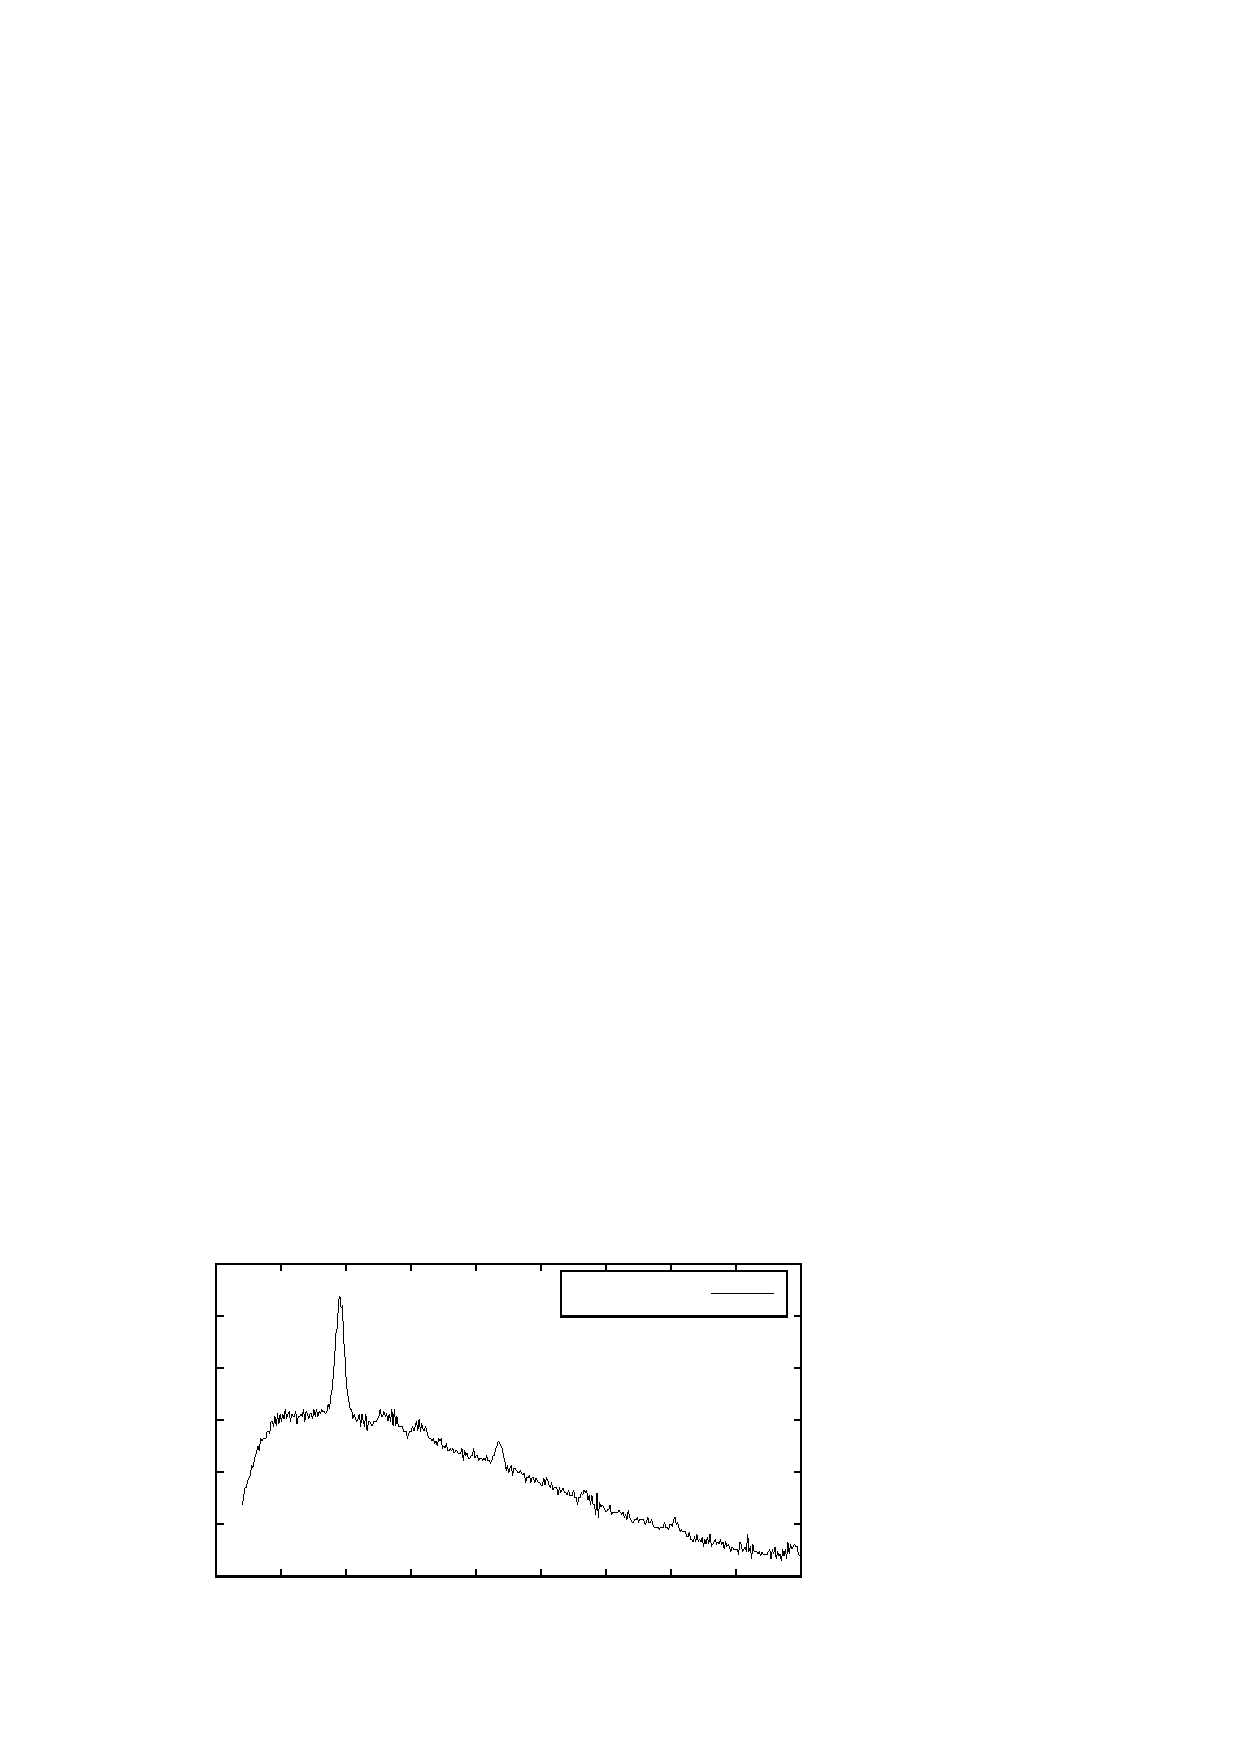
\includegraphics{spec}}%
    \gplfronttext
  \end{picture}%
\endgroup

		\caption{Farbverlauf aus dem in Abbildung \ref{fig:ausschnitt} markierten Bereich}
		\label{fig:spec}
	\end{figure}

	Die Schwärzung des Films erfolgt in der Regel proportional zur Aufnahmezeit und Intensität, wenn wir Überbelichtung vermeiden.
	Aus der Bragg-Bedingung folgt, dass kleinere Wellenlängen weniger stark abgebeugt werden als große, was wiederum impliziert, dass man die x-Achse in Abbildung \ref{fig:spec} qualitativ als verzerrte Darstellung der Wellenlänge ansehen kann.
	Hohe Intensitäten bedeuten stärkere Schwärzung und sind deshalb mit geringeren Werten von \textit{ImageJ} belegt worden.
	Deshalb wurde die y-Achse invertiert und ist ebenfalls als leicht verzerrte Intensität zu begreifen.
	Demnach ergibt sich eine Art qualitatives Spektrum der Röntgenquelle.
	Ein Vergleich zeigt schnell eine gute Übereinstimmung mit dem theoretischen Verlauf wie er unter Abschnitt \ref{ssub:charakteristische_rntgenlinien} beschrieben wurde.
	Insbesondere lässt sich die $K_\alpha$-Linie gut erkennen, $K_\beta$ verschwindet wegen der, wie weiter oben bereits erklärt, wesentlich geringeren Intensität.

% section messwerte